\documentclass[Arkitektur/System_main.tex]{subfiles}
\begin{document}

\subsection{Domænemodel} \label{sec:domainmodel}

I det følgende er systemets Use Cases analyseret, med det formål at lave en model, som viser systemets domæne. Domænemodellen i figur \ref{fig:domain_model} giver et overblik over, hvilke elementer der indgår i Beerpong Table's software. Det illustrerer systemets funktion på et mere overordnet, konceptuelt plan og viser hvilke elementer, som senere skal designes og implementeres. Det fremgår af figur \ref{fig:domain_model}, hvordan servicemedarbejder interagerer med Ball dispenser, mens bruger primært interagerer med kop og WebPage. Derudover ses det bl.a., at RPi er afgørende for afviklingen af WebPage, herunder Scoreboard og Game History, samt kommunikationen med PSoC i Player side. 

\begin{figure}[H]
    \centering
    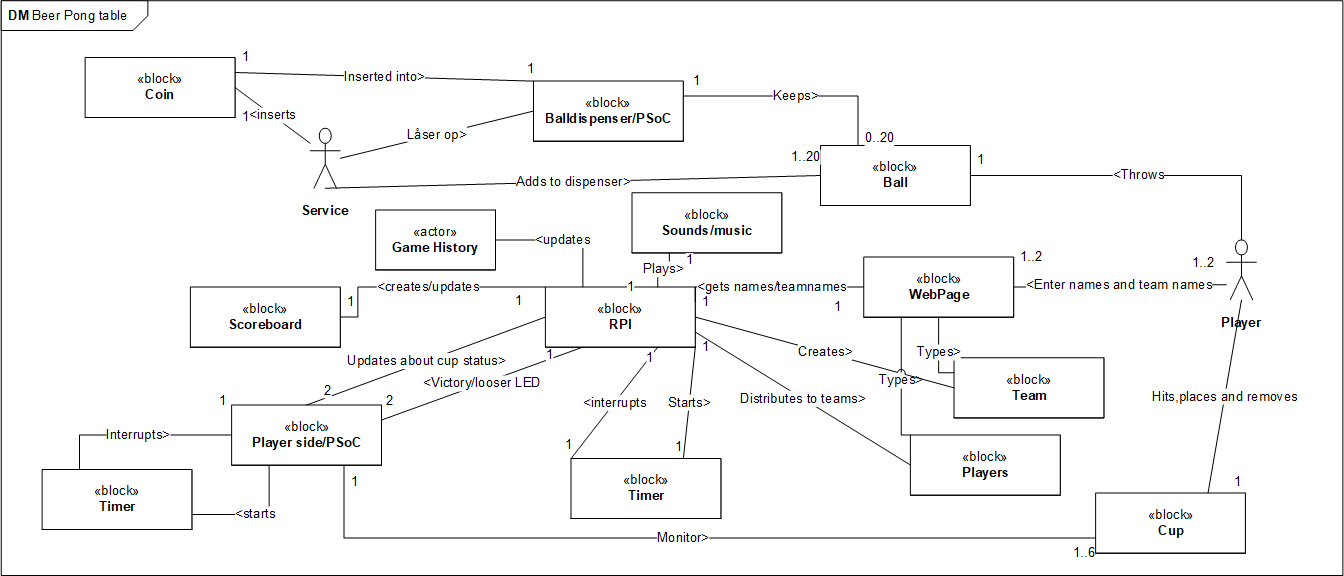
\includegraphics[angle=90, scale=0.7]{Arkitektur/Softwarearkitektur/Domaenemodel/graphics/domain_model.png}
    \caption{Domænemodel for Beerpong Table}
    \label{fig:domain_model}
\end{figure}

\end{document}